% Framework overview (raster, 2026-10-25; replaces the B1-only TikZ overview kept in figs/fig_overview_b1_tikz.tex).
% 2026-10-27: material column relabelled (external appearance backend + planned constrained fusion) and a status note for G,
% by figs/src/relabel_framework.py from the user's original figs/src/fig_overview_framework_user.png.
% The caption states which boxes produce the results reported in this paper and which are under test, negative or planned.
\begin{figure*}[t]
\centering
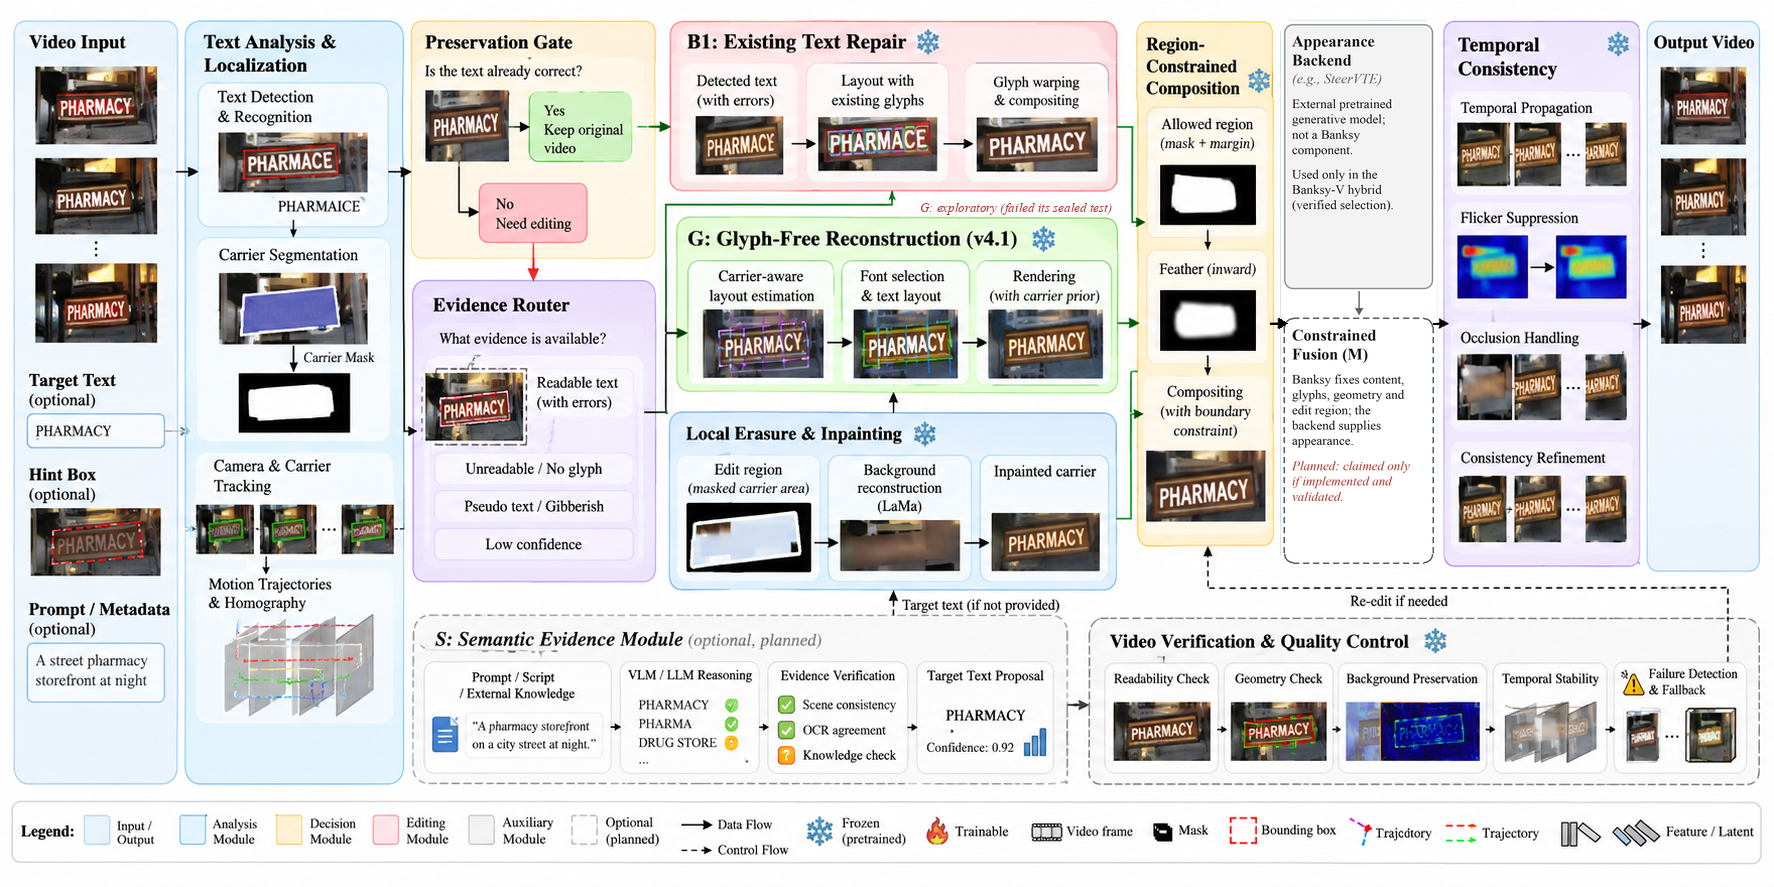
\includegraphics[width=\linewidth]{figs/fig_overview_framework.png}
\caption{\textbf{\method framework and the scope of this paper.} Text analysis reads and tracks the text and its carrier; the preservation gate returns the clip unchanged when the text already reads the target; otherwise the evidence available decides between repairing the existing text (B1) and glyph-free reconstruction (G); local erasure and a region-constrained compositor keep every edit inside the allowed region. \emph{Status:} all reported results come from the frozen B1 path; its only appearance step is the non-parametric source appearance transport, nothing is trained, and of the temporal box only carrier-anchored propagation belongs to it. G failed its sealed test and is exploratory (\cref{sec:exp_neg}). The appearance backend is an external model~\cite{zeng2026steervte} used only in Banksy-V (\cref{sec:exp_hybrid}); M, S, the router and the verification loop are planned, and a trained material generator was negative.}
\label{fig:overview}
\end{figure*}
